\documentclass[a4paper,12pt,,titlepage,openright]{report}


%-------PACKAGE-------
\usepackage[utf8]{inputenc}
\usepackage[T1]{fontenc}
\usepackage{indentfirst}
\usepackage{microtype}
\usepackage[english]{babel}
\usepackage{verbatim}
\usepackage{setspace}
\usepackage{subfig}
\usepackage{graphicx}
\usepackage{geometry}
\geometry{a4paper,top=3cm,bottom=3cm,left=3cm,right=3cm, heightrounded,bindingoffset=5mm}
\onehalfspacing
\usepackage{graphicx}
\usepackage{fancyhdr}
\usepackage{fancyvrb}
%\usepackage{showkeys}
\usepackage{mathtools}
%\usepackage[nolabel]{showlabels}
\usepackage{amsmath}
\usepackage{graphicx}
\usepackage{listings}
\usepackage{quoting}
\usepackage[nottoc]{tocbibind}
\usepackage{hyperref}
\usepackage{booktabs}
\usepackage[square,sort,comma,numbers]{natbib}
\usepackage{acronym}
\newcommand\tab[1][1cm]{\hspace*{#1}}

\pagestyle{fancy}\addtolength{\headwidth}{20pt}
   \renewcommand{\chaptermark}[1]{\markboth{\thechapter}{}}
   \renewcommand{\sectionmark}[1]{\markright{\thesection}{}}
   \cfoot{}
   \rhead[\fancyplain{}{\bfseries\leftmark}]{\fancyplain{}
                                           {\bfseries\thepage}}
   \lhead[\fancyplain{}{\bfseries\thepage}]{\fancyplain{}
                                         {\bfseries\rightmark}}
                                         
                  

\makeatletter
\renewenvironment{thebibliography}[1]
     {\section*{\refname}%
      \@mkboth{\MakeUppercase\refname}{\MakeUppercase\refname}%
      \list{}%
           {\setlength{\labelwidth}{0pt}%
            \setlength{\labelsep}{0pt}%
            \setlength{\leftmargin}{\parindent}%
            \setlength{\itemindent}{-\parindent}%
            \@openbib@code
            \usecounter{enumiv}}%
      \sloppy
      \clubpenalty4000
      \@clubpenalty \clubpenalty
      \widowpenalty4000%
      \sfcode`\.\@m}
     {\def\@noitemerr
       {\@latex@warning{Empty `thebibliography' environment}}%
      \endlist}
\makeatother                  
                                         
\makeindex                                                                            

\begin{document}
\title{\textbf{\Huge {Python to C compiler}}
\\
\begin{figure}[htbp]
\centering

\includegraphics[width=1.1\textwidth]{pytoc.png}
\end{figure}}

\author{Piergiorgio Ladisa \\
Mat. [573036]}
\maketitle
\tableofcontents
\listoffigures

\chapter{Introduction to the Python to C compiler}
\section{Python}
\textbf{Python} was created during the early '90s by Guido van Rossum as a successor of the language known as ABC and distribuited under a GPL-compatible licence and so all the releases of Python can be considered Open Source. Since those years, the language has undergone continuous developments.
Python is a powerful high-level programming language, born to combine the advantages of scripting with those of structured programming. Often happens to have the need to add more functions to a large script: this could weigh it down considerably. It may also happens to want to add features that are only accessible via C, as the system-call.
Therefore, Python starts to be an interpreted language and this speeds up the development of the program as it avoids the compiling and linking phases; nevertheless it offers many more facilities and support for big programs despite of shell languages. Python also allows to split the program in reusable modules and to write them in a more compact way. In this way, the program results to be easier to read for these reasons:
\begin{itemize}
\item high-level data types allow to express complex operations in few instructions;
\item instructions are not grouped by parenthesis but through indentation;
\item it is not necessary to declare variables.
\end{itemize}
Finally, one of Python's greatest potential is to be \textit{extensible}: it is possible to add to the interpreter new functions or built-in modules to execute critical operations in a fast manner or to create links to libraries.

\section{C}
\textbf{C} is a general-purpose programming language, developed by Dennis M. Ritchie and Brian W. Kernighan. The main important ideas at the basis of C stem from the languages BCPL and then the language B.
The language C provides a variety of data types. The fundamental types are characters, integers, floating point and then some derived data types created with pointers, arrays, structures and unions. The expressions are formed by operators and operands; C also provides the fundamental control-flow constructions required for \textit{well-structured programs} as statement grouping, decision making (if-else), looping with tests (while, for, do-while) and selecting of a set of possible cases (switch). C also provides the feature to define functions that can be called when they are needed. 
Functions of a C program may exist in separate source files that are compiled separately and a preprocessing step performs macro substitution on program text, inclusion of other source files and conditional compilation.
Therefore, C is a relatively "low level" language, that it means that C deals with the same sort of objects that most computers do, namely characters, numbers but also addresses: in this way, programmer can also go down to memory level and manage low-level details.

\section{Python to C compiler}
The compiler realized as a project is a \textit{source-to-source compiler} that translates a Python 2.7 program into a C program.
The steps to perform the translation are the following:
\begin{enumerate}
\item the \textbf{lexical analyzer} reads the character stream from the source program written in Python and tokenizes it. In this step I utilized the tool \textbf{Flex}, with which I defined the regular expressions for the patterns that identify \textit{identifiers, strings, reserved words of Python language, integers, floating points, strings and symbols of arithmetical and conditional expressions}, and for each one a token is generated.
For what concerns identifiers, they are stored  in the symbol table. At the same time, values of integers, floating points and strings are stored into the global variable \textbf{yylval}. In this way, the scanner and the parser can share not only symbols, but also their values;
\item a \textbf{syntactic analyzer} that receives as input the string of tokens from the scanner, verifies if the string of tokens can be accepted from the grammar defined and, if everything is correct, generates as its output the \textbf{abstract syntax tree}. The tool utilized in this step is the parser generator known as \textbf{Bison};
\item finally, a \textbf{semantic analyzer} evaluates the tree to generate the target program in C or to check if semantical errors occur. In this step I didn't use any tools, but it was all written by hand as external routines called by Bison during the parsing process.
\end{enumerate}
The following figure shows the block diagram of the system.
\begin{figure}[htbp]
\centering
\includegraphics[width=1\textwidth]{blockdiagram.png}
\caption{Block diagram of Python to C compiler}
\end{figure}

\chapter{Description of the project}
\section{Restriction on the source language}
Since the design of a compiler for an entire language is a long and laborious process, the following restriction on Python language was decided for my project:
\begin{itemize}
\item list of statements;
\item single line comments;
\item three types of selection statements, that is \textit{if}, \textit{if-else} and \textit{if-elif-else};
\item one loop statement, that is \textit{while} construct;
\item two built-in functions, one for the input, that is \textit{raw\_input()}, and one for the output, that is \textit{print}.
\item definition of \textbf{one} user function without return option\footnote{This choice will be motivated later.}
\end{itemize}
In addition to what has been said, it has been implemented an Abstract Syntax Tree and a Symbol Table through an hash table.

\section{Symbol table}
One of the essential function of a compiler is to store the variable names used in the source program and collect all the useful information that regards them. To reach this goal it is used a \textbf{symbol table}, that is a data structure containing a record for each variable name, with appropriate fields for attributes of that name.

First of all, in my project, a \textbf{symbol} is an istance of a struct in which are recorded these informations:
\begin{itemize}
\item name of the identifier;
\item type of the identifier, that could be one of these: not-defined, void, integer, floating-point and a string;
\item value of the identifier;
\item a flag that specifies if that identifier belongs to a general scope or to that of a function: if this flag is setted to 1, it belongs to the user-function, otherwise to the main-scope;
\item pointer to the AST of the function to which the variable belongs.
\end{itemize}
The symbol table is defined as an array of fixed size, setted to $NHASH = 9999$, and contains one routine, \textbf{lookup(char *name)}, which takes as input the name of the symbol and returns the address of that name or creating a new entry if there isn't one already.
It is important to observe that the lookup technique is known as \textit{hashing with linear probing}: it uses an hash function to transform the string in input into an entry number in the table, then checks the entry and, if it is already taken by a different symbol, scans linearly until it finds a free entry.
The hash function multiplies for each character the previous hash by $9$ and then $xor$ the character, doing all the arithmetic as unsigned, which ignores overflows.

\section{Scanner using Flex}
As I previously said, the first step of the translation process is the \textit{lexical analysis}. The latter is done by an element called \textbf{scanner}: this divides the stream of character into meaningful blocks called \textbf{token}.
So, to generate a scanner, has been used the tool known as \textit{Flex}.
A Flex program has the following form:
\begin{flushleft}
\texttt{declarations
\\
\%\% 
\\translation rules
\\
\%\%
\\auxiliary functions }
\end{flushleft}

In the \textbf{declarations part} have been included all the needed libraries such as the standard libraries for the C preprocessor, the header generated by Bison for the parser, and two important header files:
\begin{enumerate}
\item one containing the declarations of the symbol table (declared as \textit{extern} to make it accessible from extern modules) and the ASTs
\item the other one containing the declaration of a stack and the init, pop, push and pick routines to manage and solve the \textbf{indentation problem}
\end{enumerate}

The \textbf{translation rules} have the form of:
\begin{flushleft}
\texttt{ Pattern		\tab\{Action\} }
\end{flushleft}
Each \textit{Pattern} is a \textbf{regular expression} while the \textit{Action} is a C code section in which it has to be indicated what action must be taken when the pattern is encountered from the scanner.
In my project, the regular expressions match the following tokens:
\begin{itemize}
\item identifiers, that is variables or name for functions;
\item integer literals;
\item floating point literals;
\item string literals;
\item single character operators, that is +,-,*,/,=,:,(,) and comma;
\item comparison operators, that is >,<,!=,==,>=,<= 
\item keywords of Python; in particular all the reserved words have been declared because these words cannot be used as identifiers; so for correctness, the compiler must warn the programmer if he's trying to use them as a name for a variable or a function. Obviously, for the constructs or statements implemented in the project, the actions for that specific reserved words returns a token, rather than a warning message;
\item \textbf{indentation}, \textbf{dedentation} and \textbf{end of statement};
\item comments, that will be ignored.
\end{itemize}

The \textbf{auxiliary functions} part  is void.

So, the Flex-generated scanner reads through its input, matches it against all of the regular expressions and does the appropriate action on each match. In conclusion, the tool translates all of the regular expressions into an efficient internal form, that is a \textbf{Deterministic Finite Automata}.

\subsection{The "indentation problem"}
A Python program uses the indentation and the dedentation to delimit a block of code and, in a list of statements, the \textit{newline} character indicates the end of a statement. 
This features of Python language gives to it the advantage to be easier to read. But the main problem, from a lexical and a syntactical analysis point of view, is that now we are not managing a "context-free grammar" but, in such a way, a "context-sensitive grammar".
To better understand the problem let us consider C. In this language, for example, the block of statements is delimited by \{ and \}, while all the newlines and tab characters are ignored. In this case, we can generate a token everytime we encounter the characters \{ and \} and consider every statement contained between these two as a block of code.

In Python, a program is divided into a certain number of \textit{logical lines}. The end of a logical line is represented by a token that matches the new-line character, called \textit{END\_OF\_STATEMENT}.
The blank line, a logical line that contains only spaces, tabs, formfeeds and comment, is ignored.

So, how to scan the indentation, the end of a statement into a block of code, and the end of a block, that is a dedentation?
The main idea is based on the use of a stack and as follows.
The first value pushed into the stack is $0$. While a new line is encountered in a list of statements, the token generated is an END\_OF\_STATEMENT. If it begins a new block of code that is, for example, in this case:

\begin{flushleft}
\texttt{
if (x<0):
\\ \tab print "Hello world!" }
\end{flushleft}

the current value of indentation is pushed into the stack, defining the new \textbf{indentation level}. From this moment on, for every statement is checked if it is at:
\begin{itemize}
\item higher indentation level, then the new value is pushed into the stack, an INDENT token is generated and a new code-block begins;
\item lower indentation level, then the current value is popped from the stack, a DEDENT token is generated and the current code-block ends;
\item same indentation level, then an END\_OF\_STATEMENT token is generated and we are still in the same code-block.
\end{itemize}

\section{Abstract syntax tree}
In an \textbf{abstract syntax tree} each interior nodes represent programming constructs.
\begin{figure}[htbp]
\centering
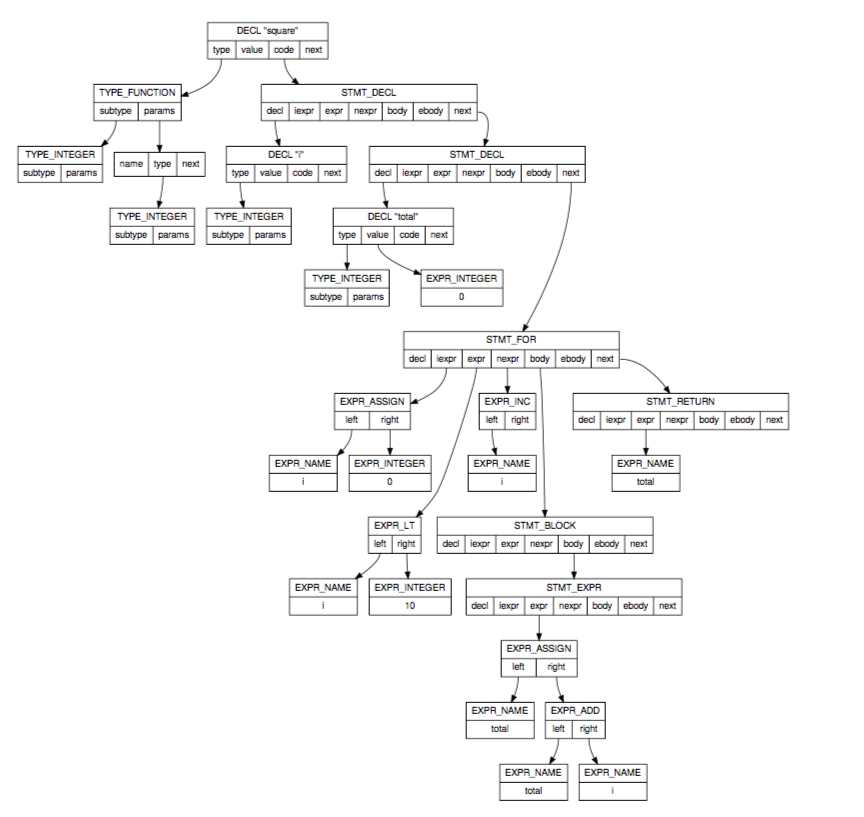
\includegraphics[width=.7\textwidth]{ast.png}
\caption{Example of an AST of a program}
\end{figure}
\\
In particular, in my project the nodes of the ASTs can be of three type:
\begin{enumerate}
\item \textbf{declarations} for functions. The single node of this kind contains these information: symbol associated to the identifier of the function, pointer to the AST of an expression associated (that is the creation of leaf for the identifier), pointer to the AST of the body of the function, pointer to the next declaration;
\item \textbf{statement}. Each statement-node must have a kind, that can be a declaration, a call to a function, an expression, an if-else statement or if-elif-else, a while statement, a print, an input function, an end of statement or a block of code; moreover, the structure contains the pointer to a declaration, three pointers to expressions (the first for initialization expression, the second for the expression to be evaluated and the third for the expression for increment), one pointer to the body of the statement, one pointer to the else body and finally a pointer to the next statement;
\item \textbf{expression}. One expression can be a sum, a subtraction, a multiplication, one of the six conditional expressions, an assignement or grouping inside brackets and then a variable, an integer, a floating point or a string. So, an expression-node must specify which one of these is, a pointer to the left leaf, a pointer to the right leaf and finally a symbol if it is a variable, an integer value if it is an integer, a floating point value if it is a floating point and a string if it is a string.
\end{enumerate}
The routines associated to the ASTs are the ones to create them, the ones to evaluate them and finally to free the memory allocated to create them.


\section{Parser using Bison}
While Flex recognizes the tokens inside a characters stream, \textbf{Bison} takes a grammar specified by the programmer and writes a parser that recognizes valid sentences in that grammar, building the associated \textit{parsing tree}.
Note that a \textit{parsing tree} differs from an \textit{abstract syntax tree} because the first can contain "helper" nodes that does not represent necessarily a programming construct, compared to the second one.
A Bison program has the same structure as a Flex one:
\begin{flushleft}
\texttt{declarations
\\
\%\% 
\\grammar rules
\\
\%\%
\\auxiliary functions }
\end{flushleft}
While the first and the third part have the same meaning as Flex, in the \textbf{rule section} in a Bison program the grammar rules must be defined. The grammar rules are described through the Backus-Naur and an action is associated to each of them:

\begin{flushleft}
\texttt{ Grammar rule		\tab\{Action\} }
\end{flushleft}

An example of grammar rules for conditional expression is the following:

\begin{flushleft}
\texttt{condExpression:
\newline\tab expression GT expression       
\newline\tab  | expression LT expression       
\newline\tab  | expression GE expression        
\newline\tab | expression LE expression                                          
\newline\tab | expression EQ expression        
\newline\tab | expression NE expression        
\newline\tab ;
}
\end{flushleft}
Here the \textbf{head} of the rule (or the \textbf{left-hand side}) is the nonterminal \textit{condExpression} while the \textbf{body} of the rule is composed by all the possible sequences of terminals (that is the token GT, LT, GE, LE and so on) and nonterminals (that is expression).

For each grammar rule, the corresponding action in my project creates the specific node of the AST, except for the start symbol \textit{program}, that exit from the program if the parsing process finished successfully, and for the next rule of the start symbol, that evaluates and then frees the AST.

\subsection{The auxiliary functions section of the parser}
In this part of the Bison program of my project, I have defined all the routines declared in the helper header for management of the symbol table, that is the hash function and the lookup function, and the function for the creation of the various nodes of the AST.
Beyond this, in this section we can see two important auxiliary functions:
\begin{enumerate}
\item the \textbf{type checker routine}, that checks if the left-hand and the right-hand types of an expression are equal. This is important for the \textbf{semantic analysis} and correctness of the program.
\item the \textbf{file-merger routine}. Infact, the evaluation of the AST generates an output file, named \texttt{codepart.txt} that contains the body of the code of the target program, and, if a function has been defined, also a file named \texttt{funcpart.txt}. Once the evaluation of the AST has been completed, both the general symbol table and the function symbol table are read to generate the files \texttt{declpart.txt} and \texttt{declpart\_function.txt} with the declarations of the variables in C language. All these files must be combined in order to form a complete and correct \texttt{.c} file. So that is the job of this routine that is, reading each file line by line in the appropriate order, build the C translation of the Python program.
\end{enumerate}
The functions for the evaluation of the tree and the function to free it are defined in a separate .c file.

\section{The evaluation of the AST}
The function for the evaluation of the AST is declared inside the helper-header file named \texttt{sym\_ast\_helper.h}, defined inside the file \texttt{YAcompiler.c} and called by the parser.

The main function is the one that evaluates the statements: it accepts as input one node of a statement, and based on the type of the node it performs a specific action, generating a specific output in C language. 

In the case of an expression, an evaluating expression's AST function is called. This latter takes as input a node of the AST of an expression, call itself for the left-hand side of that expression, evaluates it generating the appropriate output, then recall itself to evaluate the right-hand side of the same expression. In this way the routine performs an \textbf{inorder traversal} and not a \textbf{postorder traversal}.

In the same way are defined the functions for the evaluation of the AST for a user-defined function, but in this case the output is printed into a separate file.

Finally, with the same logic, functions to free the memory dinamically allocated for the AST are defined.

\section{Type assignment of Python vs. Type declaration of C}
In Python it is not necessary to declare a variable and so its type, because during the assignment  it takes the type from the right-hand part of the expression.
So, in the project, this "problem" has been solved in the same way: during the assignment of a variable, inside the action of the grammar rule, the specific entry of the symbol table corresponding to that variable is updated to make equal the type of the right-hand side of the assignment and the type of that symbol.

\section{The definition of a user function}
In my project I implemented the definition of a user function, without parameters and that does not return anything. As much as it is a very strong restriction, this helped me to understand the way and also the problems in designing a compiler that let the programmer to define functions. 
Infact, every user-function must have a separate symbol table from the others.
As we said, conceptually the symbol table is a map between the name of each identifier and the symbol structure that describes it:
\newpage
\begin{figure}[htbp]
\centering
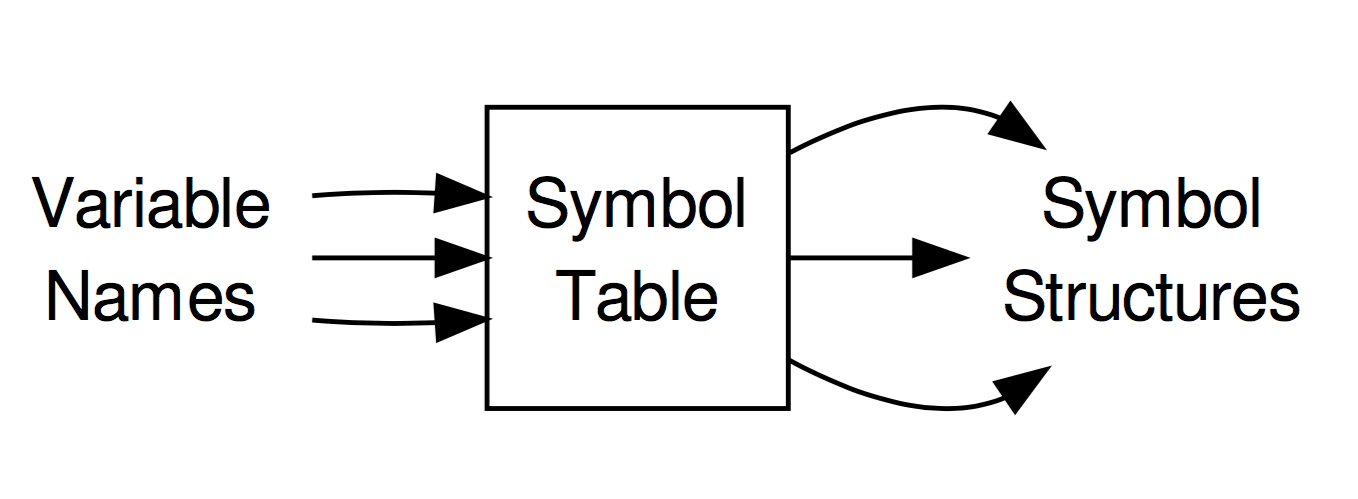
\includegraphics[width=.6\textwidth]{symboltable.png}
\caption{Symbol table}
\end{figure}
The problem occurs when the programmer wants to use the same variable name multiple times, as long as each definition in a distinct \textbf{scope} of the various functions.
To allow this feature, in the design of a compiler, it is needed to structure the symbol table as a stack of hash tables: in this way each hash table maps the names in a given scope and so it is possible to have a symbol to exist in multiple scopes, without conflict.
\begin{figure}[htbp]
\centering
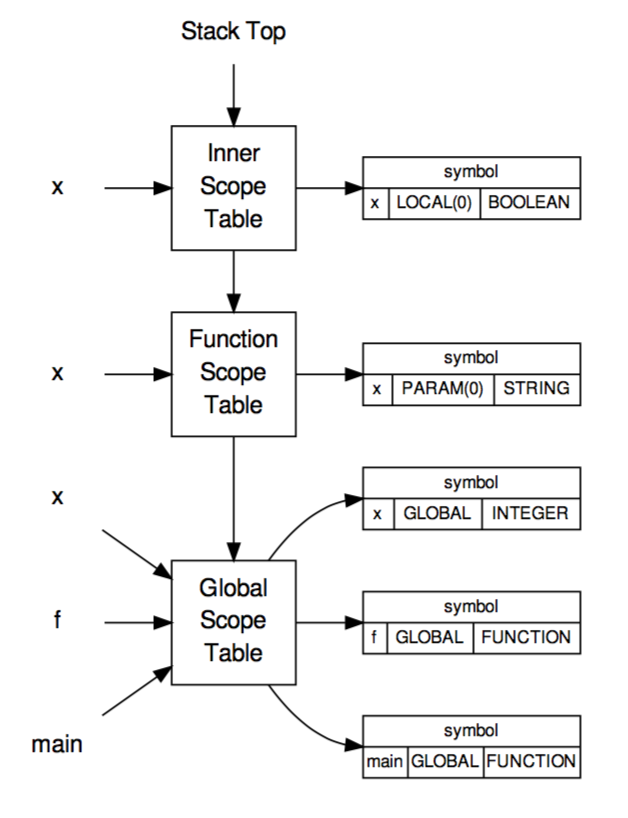
\includegraphics[width=.5\textwidth]{nestedsymbol.png}
\caption{Nested symbol table}
\end{figure}

Therefore, I decided to implement a single additional symbol table to manage the two different scopes (the global and the user-function) as a starting point for a future development of my project.

\chapter{Test cases}
Firstly, it is important to remark that the function \textbf{yyerror()} has been redefined in such a way as to print a more useful error message that indicates in which line there is the error and which kind of error occurred.
While syntactic errors are reported through the standard Bison message, the errors of type have been redesigned to indicate if a symbol has no type or if the expression is invalid because its terms have different types. Also that, if a symbol has a not-declared type the compiler warns the user to declare it.

The shell-command to generate the executable of the compiler are the following:
\begin{flushleft}
\texttt{bison -d YAparser.y
\\
flex YAlexer.l
\\
 gcc lex.yy.c YAparser.tab.c stack.c YAcompiler.c -ll -o executable.out
}
\end{flushleft}

and to execute the program, assuming to have a source file called, for example, \texttt{test.txt}:
\begin{flushleft}
\texttt{./exectuable.out < test.txt}
\end{flushleft}

The target program will be found always in the file \texttt{code.c}.
It is important to observe that it is necessary, every new compiling, to delete the files \texttt{code.c, codepart.txt, funcpart.txt, declpart.txt, declpart\_function.txt}, otherwise every output will be appended to the already existing files.
\newpage
\section{Valid source program}
\subsection{Test 1}
Let us consider the following test file:
\begin{Verbatim}
a=4
x=3
while(x>0):
	if(a==4):
		print "Hello"
		x=x-1
	else:
		print "World"
		x=x-1		
d=raw_input("Insert something")
print d
\end{Verbatim}
the output generated by the compiler is the following:
\begin{Verbatim}
#include <stdio.h>
#include <stdlib.h>
int main(void){
\* DECLARATION PART *\
int a;
char* d;
int x;
\* CODE PART *\
a=4;
x=3;
while (x>0){
if (a==4){
printf("Hello");
x=x-1;
}else{
printf("World");
x=x-1;}
}printf("Insert something");
scanf("%s",d);
printf("%s",d);
return 0;
}
\end{Verbatim}

\subsection{Test 2}
Let us consider the following test file:
\begin{Verbatim}
def funzione() :
	x=0
	if(x>=1):
		a=x*x
	else:
		a=x
print "Hello"
b=0
d=b*b
\end{Verbatim}

the output generated by the compiler is the following:
\begin{verbatim}
#include <stdio.h>
#include <stdlib.h>

void funzione(){
int a;
int x;
x=0;
if (x>=1){
a=x*x;
}else{
a=x;
}
}

int main(void){
\* DECLARATION PART *\
int b;
int d;

\* CODE PART *\
printf("ciao");
b=0;
d=b*b;
return 0;
}
\end{verbatim}

\subsection{Conclusions}
As we can see the two correct source programs are translated into two correct target programs written in C language.

\section{Invalid source program}
\subsection{Error-Test 1}
Let us consider the following test file:
\begin{Verbatim}
if(x<0)
	print "ciao"
	print d

x=5 + 3.64
\end{Verbatim}
and the error generated are these two:
\begin{Verbatim}
<Line 1> x has no type.
<Line 2> syntax error, unexpected INDENT, expecting TOKEN_COLON
Parse failed. 
\end{Verbatim}
\subsection{Error-Test 2}
Let us consider the following test file:
\begin{Verbatim}
if (x<0):
	print x

x=a 
x=5+3.64
\end{Verbatim}
and the error generated are these two:
\begin{Verbatim}
<Line 1> x has no type.
<Line 6> Invalid expression: the terms of the expression have different types.
<Line 6> a must be declared.
\end{Verbatim}

\newpage
\begin{thebibliography}{10}
\bibitem{dragon} Alfred V. Aho, Monica S. Lam, Ravi Sethi, Jeffrey D. Ullman, "Compilers: Principles, Techniques, \& Tools", 2nd Edition, Pearson and Wesley.
\bibitem{flexbison} John R. Levine, "flex \& bison", 2009, O' Reilly.
\bibitem{lexyacc} T. Niemann, "Lex and Yacc tutorial"
\bibitem{indentation} "Python Documentation" \textit{https://docs.python.org/2.7/reference/lexical\_analysis.html}
\bibitem{flexman} "Flex Manual" \textit{http://westes.github.io/flex/manual/}
\bibitem{bisonman} "Bison Manual" \textit{https://www.gnu.org/software/bison/manual/}
\bibitem{douglas} \textit{https://www3.nd.edu/~dthain/courses/cse40243/fall2016/}
\bibitem{lectures} Lectures notes of the course
\end{thebibliography}




\end{document}